\documentclass[tikz]{standalone}
\usepackage{mymacros}
\begin{document}
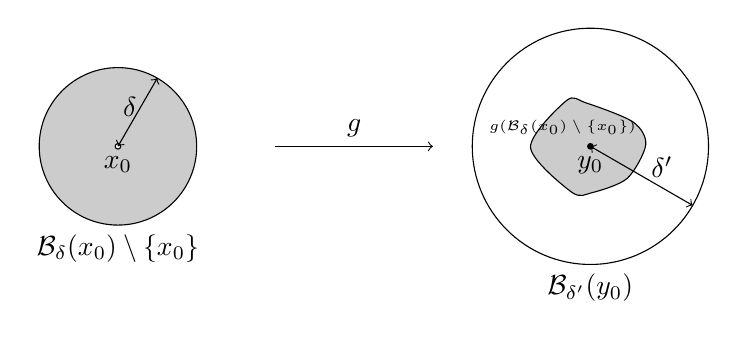
\begin{tikzpicture}    
  \colorlet{lightgray}{black!20}
  \coordinate (o1) at (-6,0);
  \coordinate (o2) at (0,0);
  \draw[->] (-4,0) -- (-2,0) node[pos=.5,above] {$g$}; % function arrow
  \draw [fill=lightgray] (o1) circle (1);
  \draw [fill=white] (o1) circle (1pt)
  node [below] {$\vect{x}_0$}; % label on top
  \draw[<->] (o1) -- ++(60:1) node[pos=.3,above] {$\delta$};
  \path (o1) ++(270:1) node [below]
  {$\mathcal{B}_{\delta} (\vect{x}_0) \setminus \left\{ \vect{x}_0 \right\}$};
  \draw (o2) circle (1.5);
  \path (o2) ++(270:1.5) node [below] {$\mathcal{B}_{\delta'} (\vect{y}_0)$};
  \pgfmathsetseed{4}
  \draw[fill=lightgray] plot [smooth cycle, samples=8,domain={1:8}]
  (\x*360/8+5*rnd:0.3cm+0.6cm*rnd) node [above left]
  {\tiny $g(\mathcal{B}_{\delta}
  (\vect{x}_0)\setminus\left\{\vect{x}_0\right\})$};
  \draw[<->] (o2) -- ++(330:1.5) node[pos=.7,above] {$\delta'$};
  \draw [fill] (o2) circle (1pt) node [below] {$\vect{y}_0$}; % label on top
\end{tikzpicture}
\end{document}


